\section{User evaluation}\label{sec:userevaluation}

We performed a preliminary, in-house user evaluation in early October. This was not a part of the original project description but we were advised by Pétur Örn Þórarinsson, our project manager, to do this before the Project Discovery game would be showcased at EVE Vegas, a conference for EVE Online players and fans. The purpose of this test was to shed light on any obvious errors with the game, especially the tutorial phase which was at an early stage at the time.

% citation á EVE Vegas http://vegas.eveonline.com/

\subsection{Implemention}
The tests took place on the 9th of October 2015. We got five participants from CCP, four males and one female between the ages of 25 to 40. The people were a mix of game designers, quality assurance people and community developers. The reason we only got people from within CCP to partake in the tests was that the game was not ready to be revealed to the public so we could not get people outside of CCP to take part.

The test was performed on a computer that remotely connected to our personal work desktop. The evaluation was performed as follows, a participant arrived, we greeted them, thanked them for coming, and explained the procedure. The procedure was that the participant would sit down and we would observe them while they played Project Discovery. The participant would open Project Discovery, finish the tutorial and a handful of other tasks. While playing, we asked the participant to think aloud . Participants could play for as long as they wanted within a reasonable amount of time, given that they continued to think aloud.

After the participant had finished playing we asked them questions about their experience playing the game and then thanked them for their contribution to the project. The questions we asked participants and their answers can be found in appendix \ref{sec.data}.

\subsection{Results}

In this section we analyze the data we derived from the tests and how we used that data to improve the game.

\subsubsection{Tooltips}
We gathered that proper use of tooltips was paramount to the players understanding of the game. Some players seemed to be confused about the objectives of the game. We saw that the tooltips needed to be clear and helpful to the players understanding the interface. So we decided that tooltips should be utilized when the players first see the interface, and also throughout the whole tutorial and training session, gradually teaching players about the game as they face the actual problems. The tooltips also needed to be shorter and focused on one specific message. Participants did not immediately grasp that they could change the color filter on the main image, so we added a tooltip that describes this functionality.

\subsubsection{Tutorial}
Participants felt that the tutorial was too easy and did not teach them very much about the real game. To rectify this we implemented a more extensive tutorial, where each task teaches the player a specific aspect of the game. Such as explaining the interface, or how to classify certain patterns in images. 

Participants expressed the need for an explanation after each tutorial task, so we reached out to the researchers at The Human Protein Atlas to get explanations for each training task, and to explain why the correct solution was correct. We also enlisted their help in making the tutorial more focused and better at teaching players the skills needed to classify images.

\subsubsection{Interface}
Participants did not have much to say about the interface with the exception of everyone being in agreement that a magnification function was necessary on the main image. We responded to that by implementing a magnification function that allows players to zoom in to the full resolution of the main image within the image container and it gives players the option to fix the position of the zoomed in image so they can easily compare the image to the categories available.

We observed that participants, who had completed the training phase, and were contributing to unknown tasks, did not get a result screen. That is normal behavior since the solution is unknown, we can not reliably give a result. We saw that when users weren't getting instant feedback they were not as interested and seemed less motivated to find the right solution to the tasks. Our solution to this problem was that since we do know the community consensus for specific tasks at any given time, we can show exact percentages for choices by other players. We felt that since participants expressed excitement in seeing a result screen, we should implement this for unknown tasks, so that the game would not lose the factor of excitement once players reach the stage of solving images that have no known solution. To achieve this, instead of giving players a confirmed correct answer like we do with training tasks, we give players the current consensus of the task at the time the user submitted his solution. This consensus screen can be seen in figure \ref{fig:consensus}. We also make sure to let players know that this consensus is not necessarily correct. That way the player can get a sense of what other players think the solution is and can see if he is in agreement with them or not.

\begin{figure}[H]
	\centering
	\graphicspath{ {./graphics/} }
	\centerline{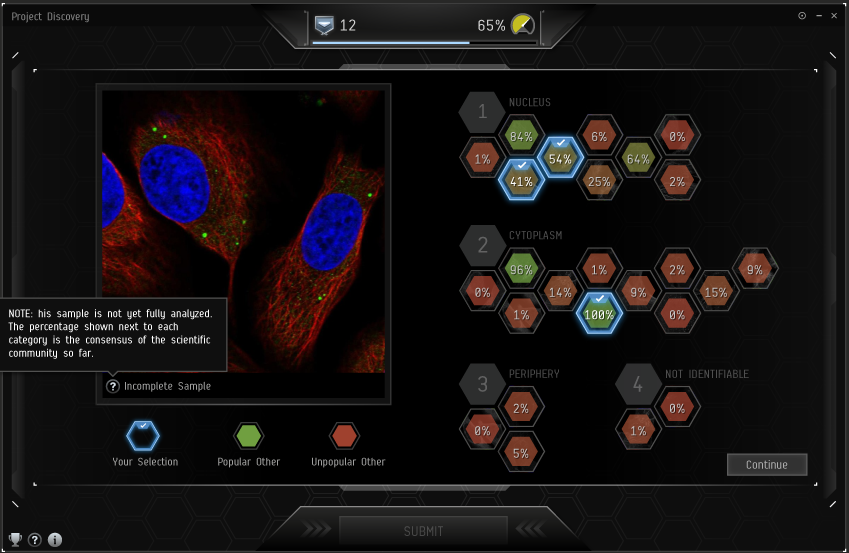
\includegraphics[scale=0.55]{unknown_result.png}}
	\caption{\label{fig:consensus}A mock-up of the consensus screen for unknown tasks}
\end{figure}

\subsection{Conclusion}

